\documentclass[conference]{IEEEtran}
\IEEEoverridecommandlockouts
% The preceding line is only needed to identify funding in the first footnote. If that is unneeded, please comment it out.
\usepackage{cite}
\usepackage{amsmath,amssymb,amsfonts}
\usepackage{algorithmic}
\usepackage{graphicx}
\usepackage{textcomp}
\usepackage{xcolor}

\usepackage{tabularx}
\usepackage{array}
\usepackage{enumitem}
\usepackage{balance}
\usepackage{comment}
\usepackage{booktabs}
\usepackage{multirow}
\usepackage{url}
\usepackage{tikz}
\usetikzlibrary{shapes.geometric, arrows.meta, positioning, fit, backgrounds, calc}
\def\BibTeX{{\rm B\kern-.05em{\sc i\kern-.025em b}\kern-.08em
    T\kern-.1667em\lower.7ex\hbox{E}\kern-.125emX}}
\begin{document}

\title{AtomicTriples: A Human-Annotated Benchmark for Triple Extraction}

\author{\IEEEauthorblockN{Rajan Lamichhane, Songhui Yue, AAA, BBB}
\IEEEauthorblockA{\textit{Department of Computer Science} \\
\textit{Charleston Southern University}\\
9200 University Boulevard, Charleston, SC 29406 \\
\{syue@csuniv.edu, rlamichhane@student.csuniv.edu\}}
}

\begin{comment}
    1) Refer to my workflow paper about the reason for selecting this code to create the triples, and combine that part here
    2) Add a workflow figure around the methodology section
    3) In Section IV, have a table that lists some examples of triple annotation for some special sentences, so that the readers know what they look like. 
    4) As long as the total page number is less than 8, it will be okay.
\end{comment}

\maketitle

\begin{abstract}
This paper presents AtomicTriples, a human-annotated benchmark for evaluating subject-predicate-object (SPO) triple extraction from ethics and professional-code text. The benchmark is built from sentences drawn from the Software Engineering Code of Ethics and Professional Practice and contains 952 manually reviewed relational triples that preserve atomic meaning, obligation, negation, and domain-specific ethical concepts. The benchmark was created by a three-person annotation workflow, supported by a custom grading tool that enabled review, voting, suggested revisions, and owner-approved final changes. We enforce 29 strict annotation rules covering atomicity, reification of complex actions, snake\_case normalization, and chain-of-action connectivity. To demonstrate the usability of the benchmark, we evaluate four extraction systems: ChatGPT, Claude, Gemini, and Stanford OpenIE. Evaluation is performed using exact string matching and soft semantic matching with embedding-based similarity thresholds. Results show that the benchmark exposes meaningful differences among systems and that revised generation rules substantially improve alignment with the human-curated gold standard. The main contribution is the benchmark itself, with an initial evaluation demonstrating how it can support repeatable comparison of triple-extraction systems.
\end{abstract}

\begin{IEEEkeywords}
triple extraction, Open Information Extraction, benchmark dataset, knowledge graph construction, annotation methodology, semantic evaluation, software engineering ethics
\end{IEEEkeywords}

\section{Introduction}
Subject-predicate-object triple extraction is a common first step in knowledge graph construction, ontology seeding, and structured knowledge representation \cite{hogan2021knowledge}. Ontology and Knowledge Graph (KG) provide a structured way to present knowledge and support reasoning \cite{vergara2023schematic}. When source text contains ethical obligations, prohibitions, professional roles, and contextual conditions, extraction quality depends on more than finding surface-level entities and verbs. A benchmark for this setting must preserve not only relational structure but also the meaning of obligation, negation, scope, and atomicity.

While significant progress has been made in Open Information Extraction (Open IE) for general-domain text \cite{angeli2015leveraging, kolluru2020openie6}, the extraction of triples from specialized professional texts presents distinct challenges. Professional ethics documents, such as codes of conduct and regulatory standards, contain dense modal constructions (e.g., ``shall,'' ``shall not,'' ``should''), layered negations, abstract professional roles, and contextual conditions that are not adequately captured by general-purpose extraction systems.

Recent advances in large language models (LLMs) have shown promising capabilities for information extraction tasks \cite{wei2023chatie, wadhwa2023revisiting}. However, evaluating these systems against structured benchmarks remains challenging, particularly when the target domain requires preservation of fine-grained semantic distinctions such as obligation versus prohibition, or when complex actions must be decomposed into atomic relational units.

This paper focuses on the benchmark rather than only the annotation framework. The purpose of AtomicTriples is to provide a human-curated gold standard that can be used to evaluate how well automated systems extract relational triples from professional ethics text. The dataset allows exact and semantic comparison of system outputs against manually validated triples. The benchmark is built from the IEEE-CS/ACM Software Engineering Code of Ethics and Professional Practice (SECEPP) \cite{acm1999code} and provides a curated gold standard of 952 triples across 110 source sentences.

SECEPP was chosen because it offers a balanced case study for ontology generation. The document is short enough to support benchmark construction while still being long enough for meaningful analysis, with a short version of 278 words and a full version of 2,653 words. Its chapter structure and list-based organization also introduce common formatting noise and processing challenges often found in software engineering standards. These features make SECEPP practical for controlled evaluation while still reflecting realistic difficulties in processing standards documents. In addition, because SECEPP focuses on ethical practice in software engineering, converting it into ontology form may support future work on ethical reasoning for software agents. This selection follows the motivation given by Yue \cite{yue2026llmrte}.

The benchmark is designed around three goals. First, each triple should express one atomic meaning. Second, the triples should preserve important ethical meaning, including obligation, prohibition, public interest, professional judgment, confidentiality, quality, and competence. Third, the dataset should be usable for evaluating both rule-based systems and LLM-based systems.

\subsection{Relates to Knowledge extraction}
Triple extraction is a specific instantiation of knowledge extraction that converts unstructured text into structured relational representations. Unlike named entity recognition (NER), which identifies entity mentions, or relation classification, which assigns labels to known entity pairs, triple extraction must simultaneously identify subjects, predicates, and objects from open-domain or domain-specific text without a predefined schema \cite{angeli2015leveraging}. The AtomicTriples benchmark targets a particularly challenging extraction setting: normative text containing modal verbs, negations, and abstract professional concepts that require careful decomposition into atomic relational units.

\subsection{Relates to Knowledge representation}
Knowledge graphs represent information as directed labeled graphs where nodes denote entities or concepts and edges denote typed relationships \cite{hogan2021knowledge}. The quality of a knowledge graph depends critically on the quality of its constituent triples. AtomicTriples contributes to knowledge representation research by enforcing strict atomicity constraints, consistent snake\_case entity naming, and reified action nodes that decompose complex verbs into structured sub-graphs. These design decisions ensure that extracted triples can be directly integrated into formal knowledge representation frameworks such as RDF or OWL.

\subsection{Related to Ontology seed construction}
Ontology construction often begins with a seed phase in which domain-relevant concepts and relationships are identified from text. Triple extraction provides a natural mechanism for ontology seeding by producing candidate classes (subjects and objects) and properties (predicates) \cite{vergara2023schematic}. The AtomicTriples benchmark is particularly relevant to ontology seeding because its source text, the Software Engineering Code of Ethics, defines professional roles, ethical principles, obligations, and organizational relationships that map directly to ontological categories. The 29 annotation rules enforce consistent entity naming and role preservation, producing triples that can serve as ontology seeds with minimal post-processing.

\subsection{LLM evaluation benchmark}
The emergence of large language models has created an urgent need for structured benchmarks that can evaluate LLM capabilities on domain-specific extraction tasks \cite{pan2024unifying}. Existing benchmarks such as OIE2016 \cite{stanovsky2016creating}, CaRB \cite{bhardwaj2019carb}, and BenchIE \cite{gashteovski2022benchie} target general-domain Open IE, while Text2KGBench \cite{mihindukulasooriya2023text2kgbench} evaluates ontology-driven knowledge graph generation. AtomicTriples fills a gap by providing a benchmark specifically designed for evaluating extraction from normative professional text, where the challenges of modality, negation, and atomicity are most acute.

The contributions of this paper are: (1)~a benchmark dataset of 110 source sentences and 952 human-curated triples; (2)~an annotation and revision process using a three-person workflow and a custom grading tool; (3)~a reproducible evaluation method using exact and semantic matching; and (4)~an empirical comparison of ChatGPT, Claude, Gemini, and Stanford OpenIE on the benchmark.


\section{Related Work}

Open Information Extraction (Open IE) aims to extract relational tuples from text without requiring a predefined schema of relations. Early systems such as ReVerb, OLLIE, and Stanford OpenIE \cite{angeli2015leveraging} relied on linguistic patterns and dependency parsing to identify candidate triples. More recent systems such as OpenIE6 \cite{kolluru2020openie6} and span-based models \cite{zhan2020span} employ neural architectures to improve coverage and precision.

\subsection{Open IE Benchmarks}
Open Information Extraction benchmarks have been developed to support reproducible comparison of extraction systems. OIE2016 \cite{stanovsky2016creating} created a large benchmark using QA-SRL-derived annotations and addressed the lack of a large independent gold standard for Open IE evaluation. CaRB \cite{bhardwaj2019carb} later improved Open IE evaluation through a crowdsourced benchmark and changes to matching and scoring. BenchIE \cite{gashteovski2022benchie} introduced a fact-based evaluation framework that groups equivalent extractions instead of relying only on token-level matching, and later work continued re-annotation efforts to reduce omissions and matching errors \cite{lamarche2024benchiefl}.

AtomicTriples differs from these benchmarks in its focus and granularity. Existing Open IE benchmarks often evaluate general-domain extractions, while this benchmark targets professional ethics and code-of-conduct language. This domain includes repeated modal verbs, negations, conditions, and abstract professional concepts. The benchmark therefore emphasizes atomic SPO structure, stable naming, reified action nodes, and explicit handling of obligations and prohibitions.

\subsection{LLMs for Knowledge Extraction}
The application of large language models to information extraction has grown rapidly. Wei et al.\ \cite{wei2023chatie} demonstrated zero-shot information extraction using ChatGPT by reformulating extraction as multi-turn question answering. Wadhwa et al.\ \cite{wadhwa2023revisiting} revisited relation extraction in the era of LLMs and highlighted the need for evaluation metrics beyond exact string matching, particularly when LLMs produce valid paraphrases that differ lexically from gold annotations. Xu et al.\ \cite{xu2023unleash} investigated few-shot relation extraction with LLMs, showing that prompt design significantly affects extraction quality.

Pan et al.\ \cite{pan2024unifying} provided a comprehensive roadmap for unifying LLMs and knowledge graphs, identifying triple extraction as a key integration point. Text2KGBench \cite{mihindukulasooriya2023text2kgbench} established an ontology-driven benchmark for evaluating LLM-based knowledge graph generation, measuring both extraction accuracy and ontology conformance. Generative approaches such as GenIE \cite{josifoski2022genie} have also shown that autoregressive generation can produce structured triples, though schema compliance remains a challenge.

These works collectively motivate the need for domain-specific benchmarks that test LLM extraction capabilities on text with rich modal, conditional, and negation structures, precisely the setting that AtomicTriples addresses.

\begin{table*}[t]
    \centering
    \caption{Overview of the consensus-guided annotation and adjudication protocol.}
    \label{tab:annotation-protocol}
    \small
    \renewcommand{\arraystretch}{1.15}

    \begin{tabularx}{\textwidth}{
        >{\raggedright\arraybackslash}p{0.18\textwidth}
        >{\raggedright\arraybackslash}p{0.25\textwidth}
        >{\raggedright\arraybackslash}X
    }
        \toprule
        \textbf{Phase} &
        \textbf{Main Activity} &
        \textbf{Purpose} \\
        \midrule

        Calibration annotation &
        Annotators independently annotated approximately 20\% of the sentences. &
        Identify major disagreement sources in triple granularity, predicate choice,
        object decomposition, clause handling, coordination, and intermediate concept use. \\

        \midrule

        Guideline discussion &
        Annotators compared pilot annotations and discussed difficult cases. &
        Establish an initial shared guideline for producing short, atomic, and
        ontology-compatible triples. \\

        \midrule

        Pilot revision &
        The pilot portion was redistributed and revised or re-annotated under the
        agreed guideline. &
        Avoid annotation drift by ensuring that the calibration portion follows the
        same guideline as the remaining dataset. \\

        \midrule

        Primary annotation &
        The full document was divided into four parts, each assigned to one primary
        annotator. &
        Produce candidate triples for all sentences under the shared annotation
        guideline. \\

        \midrule

        Dual review &
        Each candidate set was reviewed by at least two additional reviewers. &
        Ensure that each sentence involved at least three participants in the decision
        process: one primary annotator and two reviewers. \\

        \midrule

        Adjudication &
        Disagreements were resolved through majority agreement or expert discussion. &
        Produce the final gold triples and document both method-level and triple-level
        decisions. \\

        \bottomrule
    \end{tabularx}
\end{table*}

\begin{table}[t]
    \centering
    \caption{Two levels of adjudication used in benchmark construction.}
    \label{tab:two-level-adjudication}
    \small
    \renewcommand{\arraystretch}{1.15}

    \begin{tabularx}{\columnwidth}{
        >{\raggedright\arraybackslash}p{0.30\columnwidth}
        >{\raggedright\arraybackslash}X
    }
        \toprule
        \textbf{Level} &
        \textbf{Description} \\
        \midrule

        Method-level adjudication &
        Resolves disagreements about how a sentence structure should be decomposed,
        such as that-clauses, relative clauses, infinitival phrases, coordination,
        embedded conditions, and normative statements. \\

        \midrule

        Triple-level adjudication &
        Resolves disagreements about specific candidate triples, including whether
        to accept, reject, modify, or supplement a triple. \\

        \bottomrule
    \end{tabularx}
\end{table}


\subsection{Annotation Protocol}

The benchmark was constructed using a calibration-based, consensus-guided,
multi-reviewer adjudication protocol:

\begin{enumerate}
    \item \textbf{Independent calibration.}
    Annotators independently annotated approximately 20\% of the sentences.

    \item \textbf{Disagreement analysis.}
    The team compared pilot annotations and identified disagreement sources,
    including triple granularity, predicate wording, object decomposition,
    clause handling, and the use of intermediate concepts.

    \item \textbf{Guideline formation.}
    The team established an initial guideline for producing short and atomic triples.

    \item \textbf{Pilot revision.}
    The calibration portion was redistributed and revised or re-annotated under the
    agreed guideline to avoid annotation drift.

    \item \textbf{Primary annotation.}
    The full document was divided into four parts, with each part assigned to one
    primary annotator.

    \item \textbf{Dual review.}
    Each candidate triple set was reviewed by at least two additional reviewers.

    \item \textbf{Adjudication.}
    Disagreements were resolved through majority agreement or expert discussion.

    \item \textbf{Gold benchmark construction.}
    Final gold triples were produced by combining primary annotations, reviewer
    scores, reviewer suggestions, and adjudication outcomes.
\end{enumerate}

\subsection{Quality Control and Reporting}

Because atomic triple annotation is an open-ended structured generation task, we report both agreement-oriented and process-oriented quality indicators in Table~\ref{tab:quality_indicators}.

\begin{table}[htbp]
\caption{Quality and Process Indicators of the Adjudicated Benchmark}
\label{tab:quality_indicators}
\centering
\small
\begin{tabular}{lr}
\toprule
\textbf{Quality \& Process Indicator Metric} & \textbf{Value} \\
\midrule
Source sentences & 110 \\
Final gold triples & 952 \\
Average number of triples per sentence & 8.65 \\
Number of annotators and reviewers & 3 \\
Percentage of sentences in calibration phase & 20.0\% \\
Pilot-stage triple overlap / Approximate F1 & N/A \\
Reviewer agreement on candidate-triple decisions & N/A \\
Triples accepted without change & 344 (99.4\%) \\
Triples modified after review & 2 (0.6\%) \\
Rejected triples & 106 \\
Missing triples suggested \& added after adjudication & 0 \\
Method-level adjudication cases (general comments) & 1 \\
Triple-level adjudication cases (triple comments/replies) & 23 \\
Guideline updates or documented method decisions & 1 \\
\bottomrule
\end{tabular}
\end{table}


\section{Description of the Annotation Methods}


\subsection{Methodological Background: Annotation, Agreement, and Open-Ended Triple Extraction}

Human annotation is a central component in the construction of gold-standard benchmarks. In computational linguistics, inter-coder or inter-annotator agreement has been widely used to assess the reliability of human judgments \cite{artstein2008intercoder}. However, agreement measurement becomes more difficult when the annotation target is not a fixed categorical label but a structured, open-ended output. In such cases, annotators may disagree not only because one annotation is incorrect, but also because they choose different segmentation boundaries, levels of abstraction, or representation strategies.

This challenge is closely related to Open Information Extraction (OIE), where systems extract relational facts from sentences without a fixed schema. Prior OIE benchmark studies have shown that evaluation can be unreliable when gold benchmarks do not capture acceptable variants of the same fact \cite{gashteovski2021benchie}. AnnIE further demonstrates the need for interactive annotation support when constructing complete fact-oriented OIE benchmarks, because annotators must manage multiple acceptable surface realizations and difficult sentence-level extraction decisions \cite{friedrich2022annie}. These observations are relevant to our task because atomic triple annotation similarly requires annotators to convert natural-language sentences into structured subject--predicate--object representations.

Our task differs from simple relation labeling or classification-style annotation. The annotators must decide how to decompose complex normative sentences into concise triples, how to handle embedded clauses, relative clauses, infinitival phrases, coordination, and conditions, and when to introduce intermediate concepts. Therefore, a single agreement score is not sufficient to characterize the quality of the benchmark. Instead, the benchmark requires a structured process that combines calibration, guideline refinement, multi-reviewer grading, and adjudication. Recent work on complex structured and free-text annotation also highlights that traditional agreement measures are harder to interpret for complex outputs and often require task-specific matching or distance functions \cite{braylan2022measuring}. In addition, recent assessments of annotation reporting in NLP emphasize the importance of documenting annotator expertise, training, adjudication, agreement values, and other process-level details needed to assess annotation validity \cite{kunilovskaya2026who}.

\subsection{Consensus-Guided Annotation and Adjudication Protocol}

To construct the benchmark, we adopted a calibration-based, consensus-guided, multi-reviewer adjudication protocol. The goal was not only to produce a final set of gold triples, but also to make the annotation decisions traceable and consistent for an open-ended structured generation task.

In the calibration phase, annotators independently annotated approximately 20\% of the sentences. This phase was used to identify disagreements rather than to directly produce the final benchmark. The annotators compared their independently produced triples and discussed disagreements in triple granularity, predicate selection, object decomposition, clause handling, coordination, and the use of intermediate concepts. Based on these discussions, the team established an initial annotation guideline for producing short and atomic triples.

After the calibration discussion, the pilot portion was redistributed and re-annotated or revised according to the agreed guideline. This step ensured that the initial 20\% was not treated as a separate portion produced under earlier assumptions, thereby reducing annotation drift. The full document was then divided into four parts. Each part was assigned to one primary annotator, who produced candidate triples for the assigned sentences. Each candidate set was then reviewed by at least two additional reviewers. Therefore, each sentence involved at least three participants in the decision process: one primary annotator and two reviewers.

Because many disagreements concerned not only individual triples but also the appropriate extraction strategy, we resolved disagreements at two levels. At the method level, annotators discussed how newly encountered sentence structures should be handled, such as that-clauses, relative clauses, infinitival phrases, coordinated objects, and embedded normative conditions. These discussions were used to refine the annotation guideline when necessary. At the triple level, reviewers evaluated candidate triples and could accept, reject, modify, or suggest missing triples. Final gold triples were determined by combining the primary annotation, reviewer scores, reviewer suggestions, and adjudication discussions when necessary. Majority agreement was used when applicable, while expert adjudication was used for complex structural or methodological disagreements.

This process allowed the benchmark to be constructed under a shared guideline while still accommodating the open-ended nature of atomic triple annotation. It also preserved the rationale behind difficult decisions, making the resulting benchmark more transparent, auditable, and reusable.

\subsection{Artifact Availability}

To support transparency and reuse, we release the benchmark artifacts together with the final dataset. The repository includes the source sentences, the adjudicated gold triples in both JSON and CSV formats, the annotation guideline, the schema description, and examples of the upload format used by the grading tool. When appropriate, we also release anonymized review and adjudication records, including reviewer decisions, modification suggestions, and final adjudication outcomes. In addition, we provide a method decision log that documents how recurring linguistic structures, such as that-clauses, infinitival phrases, relative clauses, coordination, and embedded normative statements, were handled during annotation. These artifacts are intended to make the benchmark construction process auditable and to support future reuse or extension of the dataset.

\subsection{a Brief Description}
The benchmark was created through a manual annotation process involving a group of three annotators. The source text was based on the Software Engineering Code of Ethics and Professional Practice \cite{acm1999code}. The sentences span principle headings (e.g., ``Principle~4: JUDGMENT''), professional obligations, prohibitions, lists of enumerated duties, contextual conditions, and abstract ethical concepts. Work was divided among the annotators, who independently created triples for assigned sentences and then discussed rule differences to form a standard annotation guideline.

The annotation rules required each triple to contain a subject, predicate, and object; each row to represent one atomic relation; source sentences to remain traceable through sentence identifiers; and entities and predicates to use consistent normalized naming. The rules also required annotators to preserve negation, modality, ethical obligations, role names, and important domain concepts. The iterative process produced 29 strict rules governing triple construction.

\subsection{Annotation Rules}
The 29 annotation rules enforce the following principles:

\begin{enumerate}[leftmargin=*]
\item \textbf{Atomicity.} Each triple must express exactly one fact. Lists are split into separate triples and compound predicates are decomposed. For example, the sentence ``Software engineers shall maintain integrity and independence'' yields two triples: \texttt{(software\_engineers, shall\_maintain, integrity)} and \texttt{(software\_engineers, shall\_maintain, independence)}.

\item \textbf{Normalization.} All subjects, predicates, and objects use lowercase \texttt{snake\_case} with a maximum of three words per component and no more than three underscores per triple element.

\item \textbf{Reification.} Complex actions with targets, purposes, conditions, or results are decomposed using numbered action nodes (e.g., \texttt{influence\_001}, \texttt{consider\_broadly\_001}). This produces chain-of-action structures that maintain connectivity within a sentence's triple set.

\item \textbf{Chain of Action.} No triple may be independent within a sentence; all triples must be connected through shared entities or action nodes to preserve the sentence's semantic coherence.

\item \textbf{Modal Preservation.} Obligation verbs (``shall,'' ``should,'' ``must'') and prohibitions (``shall not,'' ``shall not knowingly use'') are preserved in predicates rather than being weakened or dropped.

\item \textbf{Negation Preservation.} Negative constructions are represented directly in predicates (e.g., \texttt{shall\_not}, \texttt{is\_not}, \texttt{not\_addressed\_by}) rather than being omitted or inverted.

\item \textbf{Role Preservation.} Professional roles such as \texttt{software\_engineers}, \texttt{client}, \texttt{employer}, and \texttt{public} are preserved exactly as entities rather than being replaced by generic terms.

\item \textbf{No Inference Beyond the Sentence.} Only information explicitly stated or directly implied by grammar is extracted. No outside knowledge, opinions, or assumptions are added.

\item \textbf{Pronoun Resolution.} Pronouns (``they,'' ``their,'' ``these'') are replaced with the clear referent from the sentence when identifiable.

\item \textbf{Structured Predicates.} Predicates use dataset-style compact relation labels (e.g., \texttt{has\_purpose}, \texttt{applies\_to}, \texttt{is\_in}) rather than full English phrases.
\end{enumerate}

The complete set of 29 rules is available in the supplementary materials and covers additional aspects including condition preservation, comparison representation, source relationships, and quality control checks.

\subsection{Grading Tool and Revision Process}
To support revision, a custom grading tool was created. In this tool, annotators could upload triple files, review other users' triples, vote on proposed changes, and suggest revisions. The owner of a triple could approve changes after review. The tool provided the following capabilities:

\begin{itemize}[leftmargin=*]
\item \textbf{Upload and Display:} Annotators could upload their triple CSV files and view them organized by sentence.
\item \textbf{Peer Review:} Each annotator could review other annotators' triples side-by-side with their own.
\item \textbf{Voting:} Annotators could vote to accept, reject, or suggest revisions for individual triples.
\item \textbf{Suggested Revisions:} Annotators could propose specific edits (e.g., splitting a non-atomic triple, correcting a predicate).
\item \textbf{Owner Approval:} The original annotator of each triple retained final approval authority over suggested changes.
\end{itemize}

Once the revisions were completed, the finalized set became the human-curated golden dataset.

Fig.~\ref{fig:workflow} presents an overview of the complete benchmark creation and evaluation workflow. Source text from the Software Engineering Code of Ethics is first segmented into 110 individual sentences. These sentences follow two parallel paths: (1)~manual annotation by a three-person team using the 29 rules, followed by peer review and revision through the grading tool, producing the 952-triple golden dataset; and (2)~automated extraction by the four evaluation systems (ChatGPT, Claude, Gemini, and Stanford OpenIE), where the LLM-based systems receive both the annotation rules and source sentences as input. The system outputs and gold standard are then compared through normalization and matching using both exact string matching and soft semantic matching to produce precision, recall, and F1 scores.

\begin{figure*}[htbp]
\centering
\resizebox{0.95\textwidth}{!}{%
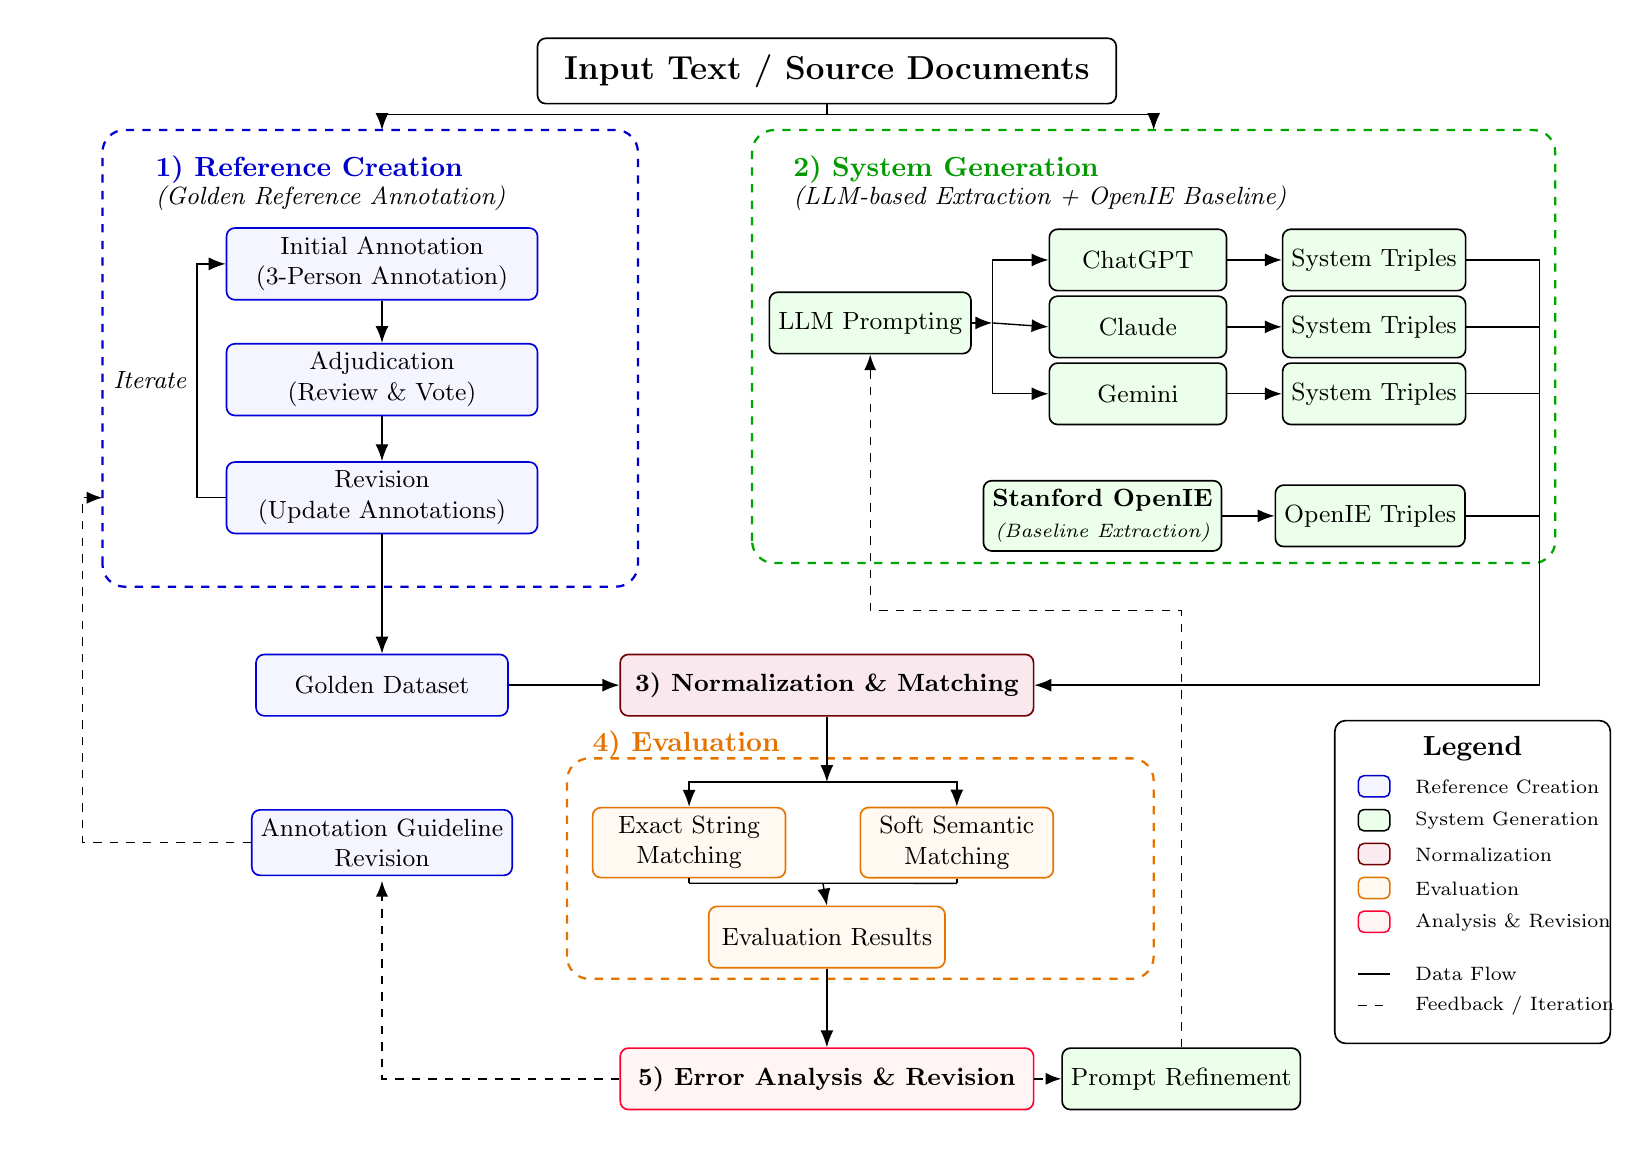
\begin{tikzpicture}[
  x=1cm,y=1cm,
  >=Latex,
  font=\small,
  data/.style={-{Latex[length=2.15mm,width=1.65mm]}, draw=black, line width=0.50pt},
  line/.style={draw=black, line width=0.50pt},
  feed/.style={-{Latex[length=2.0mm,width=1.55mm]}, draw=black, line width=0.50pt, dashed, dash pattern=on 3pt off 3pt},
  feedline/.style={draw=black, line width=0.50pt, dashed, dash pattern=on 3pt off 3pt},
  box/.style={rounded corners=3pt, draw=black, line width=0.60pt, align=center, inner sep=3.2pt, minimum height=0.78cm, fill=white},
  ref/.style={box, draw=blue!85!black, fill=blue!4, minimum width=3.95cm},
  sys/.style={box, draw=black, fill=green!8, minimum width=2.25cm},
  norm/.style={box, draw=red!45!black, fill=purple!9, minimum width=5.25cm, font=\bfseries\small},
  eval/.style={box, draw=orange!90!black, fill=orange!5, minimum width=2.45cm},
  err/.style={box, draw=red!80!magenta, fill=red!4, minimum width=5.25cm, font=\bfseries\small},
  title/.style={box, font=\bfseries\large, minimum width=7.35cm, minimum height=0.83cm},
  group/.style={dashed, dash pattern=on 3pt off 3pt, rounded corners=8pt, line width=0.82pt}
 ]

\path[use as bounding box] (-0.55,-0.65) rectangle (19.45,13.35);

% Top input
\node[title] (input) at (9.60,12.80) {Input Text / Source Documents};

% Group boundaries
\draw[group, blue!80!black] (0.40,6.25) rectangle (7.20,12.05);
\draw[group, green!65!black] (8.65,6.55) rectangle (18.85,12.05);
\draw[group, orange!90!black] (6.30,1.27) rectangle (13.75,4.07);

% Titles
\node[anchor=west, text=blue!80!black, font=\bfseries\normalsize] at (0.95,11.55) {1) Reference Creation};
\node[anchor=west, font=\itshape\small] at (0.95,11.18) {(Golden Reference Annotation)};
\node[anchor=west, text=green!60!black, font=\bfseries\normalsize] at (9.05,11.55) {2) System Generation};
\node[anchor=west, font=\itshape\small] at (9.05,11.18) {(LLM-based Extraction + OpenIE Baseline)};
\node[anchor=west, text=orange!90!black, font=\bfseries\normalsize] at (6.50,4.25) {4) Evaluation};

% Reference creation
\node[ref] (initial) at (3.95,10.35) {Initial Annotation\\(3-Person Annotation)};
\node[ref] (adj) at (3.95,8.88) {Adjudication\\(Review \& Vote)};
\node[ref] (rev) at (3.95,7.38) {Revision\\(Update Annotations)};
\node[ref, minimum width=3.20cm] (gold) at (3.95,5.00) {Golden Dataset};
\node[ref, minimum width=3.20cm] (guide) at (3.95,3.00) {Annotation Guideline\\Revision};

\draw[data] (initial.south) -- (adj.north);
\draw[data] (adj.south) -- (rev.north);
% Refined iterate loop
\coordinate (iterL1) at (1.60,7.38);
\coordinate (iterL2) at (1.60,10.35);
\draw[data] (rev.west) -- (iterL1) -- (iterL2) -- (initial.west);
\node[font=\itshape\small] at (1.00,8.88) {Iterate};

% System generation
\node[sys, minimum width=2.45cm] (llm) at (10.15,9.60) {LLM Prompting};
\node[sys] (gpt) at (13.55,10.40) {ChatGPT};
\node[sys] (claude) at (13.55,9.55) {Claude};
\node[sys] (gemini) at (13.55,8.70) {Gemini};
\node[sys] (st1) at (16.55,10.40) {System Triples};
\node[sys] (st2) at (16.55,9.55) {System Triples};
\node[sys] (st3) at (16.55,8.70) {System Triples};
\node[sys, minimum width=3.00cm] (openie) at (13.10,7.15) {\textbf{Stanford OpenIE}\\{\itshape\scriptsize (Baseline Extraction)}};
\node[sys] (ot) at (16.50,7.15) {OpenIE Triples};
\node[sys, minimum width=2.85cm] (pref) at (14.10,0.00) {Prompt Refinement};

% LLM and OpenIE flows
\coordinate (llmsplit) at (11.70,9.60);
\draw[data] (llm.east) -- (llmsplit);
\draw[data] (llmsplit) |- (gpt.west);
\draw[data] (llmsplit) -- (claude.west);
\draw[data] (llmsplit) |- (gemini.west);
\draw[data] (gpt.east) -- (st1.west);
\draw[data] (claude.east) -- (st2.west);
\draw[data] (gemini.east) -- (st3.west);
\draw[data] (openie.east) -- (ot.west);

% Right output bus
\coordinate (busTop) at (18.65,10.40);
\coordinate (busMid) at (18.65,9.55);
\coordinate (busLow) at (18.65,8.70);
\coordinate (busOpen) at (18.65,7.15);
\coordinate (busBottom) at (18.65,5.00);
\draw[line] (st1.east) -- (busTop);
\draw[line] (st2.east) -- (busMid);
\draw[line] (st3.east) -- (busLow);
\draw[line] (ot.east) -- (busOpen);
\draw[line] (busTop) -- (busBottom);

% Normalization, evaluation, error analysis
\node[norm] (norm) at (9.60,5.00) {3) Normalization \& Matching};
\node[eval] (exact) at (7.85,3.00) {Exact String\\Matching};
\node[eval] (soft) at (11.25,3.00) {Soft Semantic\\Matching};
\node[eval, minimum width=3.00cm] (res) at (9.60,1.80) {Evaluation Results};
\node[err] (err) at (9.60,0.00) {5) Error Analysis \& Revision};

% Input branching - clean downward arrowheads only
\coordinate (topJunction) at (9.60,12.25);
\coordinate (leftDropTop) at (3.95,12.25);
\coordinate (rightDropTop) at (13.75,12.25);
\draw[line] (input.south) -- (topJunction);
\draw[line] (topJunction) -- (leftDropTop);
\draw[line] (topJunction) -- (rightDropTop);
\draw[data] (leftDropTop) -- (3.95,12.05);
\draw[data] (rightDropTop) -- (13.75,12.05);

% Main cross-section data flows
\draw[data] (rev.south) -- (gold.north);
\draw[data] (gold.east) -- (norm.west);
\draw[data] (busBottom) -- (norm.east);

% Normalization to matching: one vertical then split
\coordinate (splitEval) at (9.60,3.77);
\draw[data] (norm.south) -- (splitEval);
\draw[data] (splitEval) -| (exact.north);
\draw[data] (splitEval) -| (soft.north);

% Evaluation to results (clean vertical merge)
\coordinate (mergeLeft) at ($(exact.south)+(0,-0.06)$);
\coordinate (mergeRight) at ($(soft.south)+(0,-0.06)$);
\coordinate (mergeMid) at ($(mergeLeft)!0.5!(mergeRight)$);
\draw[line] (exact.south) -- (mergeLeft);
\draw[line] (soft.south) -- (mergeRight);
\draw[line] (mergeLeft) -- (mergeRight);
\draw[data] (mergeMid) -- (res.north);
\draw[data] (res.south) -- (err.north);

% Feedback flows
\draw[feed] (pref.north) -- (14.10,5.95) -- (10.15,5.95) -- (llm.south);
\draw[feed] (err.east) -- (pref.west);
\coordinate (guideIn) at ($(guide.south)+(0,-0.06)$);
% Refined feedback from stage 5 to annotation guideline revision
\coordinate (guidePathLeft) at (3.95,0.00);
\draw[feed] (err.west) -- (guidePathLeft) -- (guideIn);
\draw[feed] (guide.west) -- (0.15,3.00) |- (0.40,7.38);

% Legend
\draw[rounded corners=4pt, line width=0.60pt] (16.05,0.45) rectangle (19.55,4.55);
\node[font=\bfseries\normalsize] at (17.80,4.20) {Legend};
\draw[rounded corners=2pt, draw=blue!80!black, fill=blue!4, line width=0.55pt] (16.35,3.58) rectangle (16.75,3.85);
\node[anchor=west, font=\scriptsize] at (16.95,3.71) {Reference Creation};
\draw[rounded corners=2pt, draw=black, fill=green!8, line width=0.55pt] (16.35,3.15) rectangle (16.75,3.42);
\node[anchor=west, font=\scriptsize] at (16.95,3.28) {System Generation};
\draw[rounded corners=2pt, draw=red!45!black, fill=purple!8, line width=0.55pt] (16.35,2.72) rectangle (16.75,2.99);
\node[anchor=west, font=\scriptsize] at (16.95,2.85) {Normalization};
\draw[rounded corners=2pt, draw=orange!90!black, fill=orange!5, line width=0.55pt] (16.35,2.29) rectangle (16.75,2.56);
\node[anchor=west, font=\scriptsize] at (16.95,2.42) {Evaluation};
\draw[rounded corners=2pt, draw=red!80!magenta, fill=red!4, line width=0.55pt] (16.35,1.86) rectangle (16.75,2.13);
\node[anchor=west, font=\scriptsize] at (16.95,1.99) {Analysis \& Revision};
\draw[line width=0.58pt] (16.35,1.33) -- (16.75,1.33);
\node[anchor=west, font=\scriptsize] at (16.95,1.33) {Data Flow};
\draw[line width=0.58pt, dashed, dash pattern=on 3pt off 3pt] (16.35,0.93) -- (16.75,0.93);
\node[anchor=west, font=\scriptsize] at (16.95,0.93) {Feedback / Iteration};

\end{tikzpicture}
}
\caption{Overview of the AtomicTriples benchmark creation and evaluation workflow. Source text is processed through manual annotation (producing the golden dataset) and automated extraction systems, with outputs compared via exact and semantic matching.}
\label{fig:workflow}
\end{figure*}

\section{Benchmark Dataset}

The benchmark contains 110 source sentences and 952 gold triples, with an average of 8.65 triples per sentence. Each triple is linked to a sentence identifier and contains a subject, predicate, and object. Table~\ref{tab:dataset_stats} summarizes the dataset statistics.

\begin{table}[htbp]
\caption{AtomicTriples Benchmark Dataset Statistics}
\label{tab:dataset_stats}
\centering
\begin{tabular}{lr}
\toprule
\textbf{Measure} & \textbf{Value} \\
\midrule
Source sentences & 110 \\
Gold-standard triples & 952 \\
Average triples per sentence & 8.65 \\
\bottomrule
\end{tabular}
\end{table}

The source sentences include principle headings, professional obligations, prohibitions, lists, contextual conditions, and abstract ethical concepts. The benchmark therefore includes both simple triples, such as principle classification triples, and more complex reified structures for actions, judgments, and constraints. The current version of the benchmark uses short triples (with a maximum of three words per component). Medium-length and long triples represent a planned extension for future work.

The dataset encompasses several structural categories of triples:

\begin{itemize}[leftmargin=*]
\item \textbf{Classification triples:} Simple identity relations such as \texttt{(principle\_4, is, judgment)}.
\item \textbf{Obligation triples:} Modal constructions such as \texttt{(software\_engineers, shall\_maintain, integrity)}.
\item \textbf{Prohibition triples:} Negated obligations such as \texttt{(software\_engineers, shall\_not\_knowingly\_use, software\_001)}.
\item \textbf{Reified action triples:} Decomposed complex actions using numbered nodes, e.g., \texttt{(influence\_001, has\_action, consider\_broadly\_001)}.
\item \textbf{Scope and condition triples:} Contextual constraints such as \texttt{(tension\_001, is\_in, some\_situations)}.
\item \textbf{List expansion triples:} Enumerated items split from compound sentences, e.g., \texttt{(role\_001, is\_in, commerce)}, \texttt{(role\_001, is\_in, industry)}.
\end{itemize}

Table~\ref{tab:annotation_examples} presents representative examples of triple annotations from the golden dataset, illustrating how different sentence types are decomposed into atomic triples.

\begin{table*}[htbp]
\caption{Examples of Triple Annotations from the Golden Dataset}
\label{tab:annotation_examples}
\centering
\small
\begin{tabularx}{\textwidth}{p{0.7cm} >{\raggedright\arraybackslash}X >{\raggedright\arraybackslash}p{1.8cm} >{\raggedright\arraybackslash}p{2.8cm} >{\raggedright\arraybackslash}p{1.8cm} >{\raggedright\arraybackslash}p{3.0cm}}
\toprule
\textbf{ID} & \textbf{Source Sentence} & \textbf{Type} & \textbf{Subject} & \textbf{Predicate} & \textbf{Object} \\
\midrule
s010 & Principle 4: JUDGMENT & Classification & principle\_4 & is & judgment \\
\midrule
\multirow{3}{*}{s002} & \multirow{3}{=}{The list of Principles and Clauses is not exhaustive.} & \multirow{3}{=}{\raggedright Negation} & list\_001 & has & principles \\
& & & list\_001 & has & clauses \\
& & & list\_001 & is\_not & exhaustive \\
\midrule
\multirow{4}{*}{s004} & \multirow{4}{=}{The Code is not a simple ethical algorithm that generates ethical decisions.} & \multirow{4}{=}{\raggedright Negation + Reification} & code\_001 & is\_not & algorithm\_001 \\
& & & algorithm\_001 & is & ethical \\
& & & algorithm\_001 & is & simple \\
& & & algorithm\_001 & generates & ethical\_decisions \\
\midrule
\multirow{5}{*}{s005} & \multirow{5}{=}{In some situations standards may be in tension with each other or with standards from other sources.} & \multirow{5}{=}{\raggedright Scope + Condition} & situation\_001 & has\_scope & some \\
& & & standards\_001 & may\_be\_in & tension\_001 \\
& & & tension\_001 & is\_between & standards\_001 \\
& & & tension\_001 & is\_with & other\_standards \\
& & & other\_standards & is\_from & other\_sources \\
\midrule
\multirow{4}{*}{s060} & \multirow{4}{=}{Computers have a central and growing role in commerce, industry, government, medicine, education, entertainment and society at large.} & \multirow{4}{=}{\raggedright List Expansion} & computers & have & role\_001 \\
& & & role\_001 & is & central \\
& & & role\_001 & is\_in & commerce \\
& & & role\_001 & is\_in & industry \\
\bottomrule
\end{tabularx}
\end{table*}

\section{Evaluation}

\subsection{Evaluation Methodology}
Four systems were evaluated: ChatGPT, Claude, Gemini, and Stanford OpenIE \cite{angeli2015leveraging}. The three LLM-based systems were each provided with the complete set of 29 annotation rules as a system prompt, along with the 110 source sentences from the Software Engineering Code of Ethics. Each LLM was instructed to generate triples in the prescribed CSV format, following the same atomicity, naming, and structural conventions used to create the golden dataset. This setup ensures that the evaluation measures each system's ability to follow structured extraction guidelines when given explicit rules and source text. Stanford OpenIE was run with its default configuration as a non-LLM baseline, processing the same source sentences without the annotation rules.

System outputs were normalized by concatenating subject, predicate, and object; lowercasing; trimming whitespace; and handling empty components consistently. Performance was measured using micro-averaged precision, recall, and F1 over the full corpus.

Table~\ref{tab:system_triples} shows the number of triples produced by each system.

\begin{table}[htbp]
\caption{Number of Triples Extracted by Each System}
\label{tab:system_triples}
\centering
\begin{tabular}{lr}
\toprule
\textbf{System} & \textbf{Triples} \\
\midrule
ChatGPT & 846 \\
Claude & 867 \\
Gemini & 656 \\
Stanford OpenIE & 944 \\
\midrule
Gold Standard & 952 \\
\bottomrule
\end{tabular}
\end{table}

\textbf{Exact String Matching.}
Exact matching required the normalized system triple to be identical to a normalized gold triple for the same sentence. This method is strict and useful for checking whether a system reproduces the benchmark structure directly. A greedy one-to-one matching algorithm was used, where each triple could be matched at most once. This method penalizes any lexical variation, including valid paraphrases.

\textbf{Soft Semantic Matching.}
Soft semantic matching addressed cases where a system produced a valid paraphrase that was not lexically identical. Each normalized triple string was embedded using spaCy's \texttt{en\_core\_web\_lg} pipeline, which provides 300-dimensional GloVe vectors. For each sentence, an $N \times M$ cosine similarity matrix was constructed between gold triples ($N$) and system triples ($M$):

\begin{equation}
\cos(\theta) = \frac{\mathbf{v}_g \cdot \mathbf{v}_s}{\|\mathbf{v}_g\| \times \|\mathbf{v}_s\|}
\end{equation}

\noindent where $\mathbf{v}_g$ and $\mathbf{v}_s$ are the embedding vectors for the gold and system triples, respectively. A greedy bipartite matching algorithm processed pairs in descending similarity order, accepting a match if the cosine similarity exceeded a threshold $t$ and neither triple had been previously matched. Rather than choosing a single threshold, we swept across a range of thresholds from 0.50 to 0.90 in increments of 0.05. This produces precision-recall curves that reveal the tradeoff between strictness and coverage for each system.


\subsection{Evaluation Results}

\textbf{Exact-Match Results.}
Table~\ref{tab:exact_results} presents the exact-match evaluation results. Exact-match performance improved for all systems. Claude achieved the strongest exact-match result with F1~=~0.3079, substantially outperforming all other systems. This result indicates that Claude's outputs most closely replicated the benchmark's lexical structure and naming conventions. ChatGPT, Gemini, and Stanford OpenIE improved but remained lower under exact matching, showing that strict lexical matching penalizes outputs that differ from the benchmark wording or structure.

\begin{table}[htbp]
\caption{Exact-Match Evaluation Results}
\label{tab:exact_results}
\centering
\begin{tabular}{lccc}
\toprule
\textbf{System} & \textbf{Precision} & \textbf{Recall} & \textbf{F1} \\
\midrule
ChatGPT & 0.0567 & 0.0504 & 0.0534 \\
Claude & 0.3230 & 0.2941 & 0.3079 \\
Gemini & 0.0518 & 0.0357 & 0.0423 \\
Stanford OpenIE & 0.0657 & 0.0651 & 0.0654 \\
\bottomrule
\end{tabular}
\end{table}

\textbf{Semantic Matching Results.}
Table~\ref{tab:semantic_results} presents the best semantic matching results. Semantic matching produced higher best F1 scores for ChatGPT, Gemini, and Stanford OpenIE. ChatGPT achieved the highest semantic F1 at 0.2792, followed closely by Gemini at 0.2786. Claude achieved 0.2672, and Stanford OpenIE achieved 0.2162. All systems reached their best semantic F1 at threshold 0.50. Notably, Gemini achieved the highest semantic precision (0.3415), suggesting that while it produced fewer triples overall (656 compared to 846 to 944 for other systems), a higher proportion of its outputs were semantically aligned with the gold standard.

\begin{table}[htbp]
\caption{Best Semantic Matching Results ($t = 0.50$)}
\label{tab:semantic_results}
\centering
\begin{tabular}{lcccc}
\toprule
\textbf{System} & \textbf{Threshold} & \textbf{Precision} & \textbf{Recall} & \textbf{F1} \\
\midrule
ChatGPT & 0.50 & 0.2967 & 0.2637 & 0.2792 \\
Claude & 0.50 & 0.2803 & 0.2553 & 0.2672 \\
Gemini & 0.50 & 0.3415 & 0.2353 & 0.2786 \\
Stanford OpenIE & 0.50 & 0.2172 & 0.2153 & 0.2162 \\
\bottomrule
\end{tabular}
\end{table}

All systems achieved their best semantic F1 at the lowest threshold ($t = 0.50$), with monotonically decreasing performance as the threshold increased toward 0.90. Fig.~\ref{fig:f1_curve} shows the F1 score as a function of similarity threshold for all four systems.

\begin{figure}[htbp]
\centering
\includegraphics[width=\columnwidth]{new_f1_curve.png}
\caption{F1 score vs.\ semantic similarity threshold for all systems. All systems achieve peak F1 at $t = 0.50$.}
\label{fig:f1_curve}
\end{figure}

Fig.~\ref{fig:precision_curve} and Fig.~\ref{fig:recall_curve} present the precision and recall curves, respectively. Gemini maintains the highest precision across all thresholds up to approximately $t = 0.80$, while ChatGPT and Claude show the highest recall at lower thresholds. Stanford OpenIE consistently trails all LLM-based systems in both metrics.

\begin{figure}[htbp]
\centering
\includegraphics[width=\columnwidth]{new_precision_curve.png}
\caption{Precision vs.\ semantic similarity threshold.}
\label{fig:precision_curve}
\end{figure}

\begin{figure}[htbp]
\centering
\includegraphics[width=\columnwidth]{new_recall_curve.png}
\caption{Recall vs.\ semantic similarity threshold.}
\label{fig:recall_curve}
\end{figure}


\section{Discussion and Future Work}\label{SCM}

\subsection{Analysis of Results}
The results show that rule design strongly affects benchmark alignment. The revised rules improved exact and semantic F1 because they encouraged shorter, more atomic triples, stable naming, explicit negation, and reified action chains. These changes moved generated outputs closer to the human-created benchmark style.

The large gap between Claude's exact-match F1 (0.3079) and the other systems (0.04 to 0.07) indicates that Claude most closely adhered to the benchmark's naming conventions and structural patterns. This suggests that Claude's instruction-following capabilities may be particularly well-suited to rule-heavy extraction tasks where specific formatting and naming conventions must be reproduced.

The convergence of semantic F1 scores across LLM-based systems (0.27 to 0.28) at $t = 0.50$ suggests that when lexical variation is accounted for, the three LLMs perform comparably in capturing the semantic content of the gold triples. The gap narrows significantly from exact matching, confirming the observation of Wadhwa et al.\ \cite{wadhwa2023revisiting} that exact-match metrics systematically underestimate LLM extraction quality.

Stanford OpenIE's consistently lower performance across all metrics highlights the limitations of pattern-based extraction systems when applied to normative text with modal obligations, negations, and reified action structures. This finding underscores the value of LLM-based approaches for domain-specific extraction tasks.

\subsection{Challenges and Limitations}
The benchmark is strict by design, and a complete extraction can still fail to match the gold standard if it combines multiple meanings, reverses triple direction, omits a modal verb, or uses a different reified node. Therefore, low exact-match scores should not be interpreted only as extraction failure; they also reflect the difficulty of matching a highly structured benchmark.

The current evaluation uses spaCy's GloVe-based embeddings (300-dimensional, \texttt{en\_core\_web\_lg}), which capture distributional similarity but may not fully represent the semantic equivalence of domain-specific terms. Transformer-based embeddings (e.g., Sentence-BERT) could provide more nuanced similarity judgments and are a target for future work.

Additionally, the current version of the benchmark uses only short triples, with a maximum of three words per component. This design choice prioritizes atomicity and consistency but limits the expressiveness of individual triples. Supporting medium-length and long triples would enable richer relational representations at the cost of increased annotation complexity.

\subsection{Future Work}
Several directions for future work emerge from this study. In the short term, adding qualitative examples of correct and incorrect extractions would help illustrate the specific challenges that each system faces. Running an error analysis of false positives and false negatives would further clarify the nature of extraction failures and help distinguish between genuine errors and naming mismatches.

In the medium term, component-level scoring that evaluates subject, predicate, and object matches separately would identify which component contributes most to extraction errors. Developing a systematic error taxonomy covering omission errors, commission errors, granularity mismatches, and naming inconsistencies would provide a more detailed picture of system performance. Computing formal inter-annotator agreement metrics such as Cohen's Kappa would also quantify annotation consistency and establish reliability bounds for the benchmark.

An important extension is the support for medium-length and long triples. The current benchmark restricts each component to a maximum of three words, which enforces atomicity but limits the representation of more complex relational structures. Future versions of the benchmark will investigate relaxing this constraint to allow richer triple representations while maintaining annotation consistency.

In the long term, expanding the benchmark beyond the Software Engineering Code of Ethics to other professional codes (e.g., medical ethics, legal codes) and technical policy documents would test whether the annotation rules generalize across domains. Replacing GloVe-based embeddings with transformer-based sentence embeddings for semantic matching is another planned improvement that could provide more accurate similarity judgments for domain-specific terminology.


\section{Conclusion}
This paper presents AtomicTriples, a human-annotated benchmark for triple extraction from professional ethics text. The main contribution is the benchmark itself: a curated dataset of 110 sentences and 952 triples designed to preserve atomicity, ethical meaning, negation, modality, and relational structure through 29 strict annotation rules.

The evaluation demonstrates the usability of the benchmark by comparing four extraction systems with exact and semantic matching. Claude achieves the highest exact-match F1 (0.3079), while ChatGPT leads in semantic F1 (0.2792) when lexical variation is tolerated. All three LLM-based systems substantially outperform Stanford OpenIE, confirming the advantage of language model approaches for domain-specific extraction tasks. The improved results after rule revision show that carefully specified annotation and generation rules can substantially improve benchmark alignment while also revealing the remaining difficulty of structured triple extraction.

The benchmark exposes meaningful performance differences among systems and provides a foundation for future work in component-level evaluation, error analysis, medium and long triple support, and domain generalization. The dataset, annotation rules, and evaluation code will be made available to support reproducible research in structured triple extraction.


\section*{Acknowledgment}
This material is based upon work supported by the National Science Foundation under Grant No. 2451397. AI tools (OpenAI's GPT-5.x, Grammarly) were used to rephrase some passages for conciseness and grammatical correctness. The content was comprehensively reviewed and revised by the authors. No AI was used to fabricate data or results.

\balance
\bibliographystyle{IEEEtran}
%\bibliographystyle{abbrv}
%\bibliographystyle{abbrv-doi}
%\bibliographystyle{abbrv-doi-narrow}
%\bibliographystyle{abbrv-doi-hyperref}
%\bibliographystyle{abbrv-doi-hyperref-narrow}
\bibliography{reference}

\end{document}
